\begin{filecontents*}{\jobname.xmpdata}
  \Title{Software quality tracking using static product metrics}
  \Author{Santeri Suitiala}
  \Keywords{software\sep metrics\sep software quality}
  \Publisher{Aalto University}
\end{filecontents*}
\documentclass[oneside,pdfa]{aaltoseries}
\makeatletter
\@ifpackageloaded{inputenc}{%
  \inputencoding{utf8}}{%
  \usepackage[utf8]{inputenc}}
\hypersetup{hidelinks}                % Linkkien korostus pois
\makeatother
\usepackage[finnish,english]{babel}   % Kieli on englanti, tiivistelmässä suomi
\usepackage{setspace}                 % Rivivälin säätämiseksi
\usepackage{afterpage}                % Sivun taustaväri
\usepackage{apacite}		  % Lähdeluettelo (Bibtex)
\usepackage{lastpage}                  % Sivumäärä
\usepackage{hyperref}                  % Kappalereferointi
\microtypesetup{letterspace=25}       % Kannen harvaan välistykseen

\author{Santeri Suitiala}
\title{Software quality tracking using static product metrics}

\begin{document}


%%  KANSI  ---------------------------------------------

\thispagestyle{empty}
\setcounter{page}{0}  % Kansisivulle sivunumero 0

% Kansisivun marginaalit
\newgeometry{left=23.2mm,right=23.2mm,top=13.5mm,bottom=18mm}

%\pagecolor{white}\afterpage{\nopagecolor}
%{\color{black}  % Musta teksti

{\parindent0pt % Kappaleiden sisennys pois päältä
{\fontsize{11.9pt}{11.9pt}\bfseries\sffamily\lsstyle Bachelor’s Programme in Electrical Engineering}

%\color{white}  % Valkoinen teksti alkaa

\vspace{13.1mm}

\begin{spacing}{3.1}
{\fontsize{35}{35}\selectfont Software quality tracking \\using static product metrics}
\end{spacing}

\vspace{2.2mm}

\begin{spacing}{1.24}
{\fontsize{14pt}{14pt}\bfseries\sffamily\lsstyle Utilization and deployment of static software metrics in software projects}
\end{spacing}

\vspace{7.2mm}

\rule{\textwidth}{1.25pt}

\vspace{8.5mm}

{\fontsize{13.9pt}{13.9pt}\bfseries\sffamily\lsstyle Santeri Suitiala}

\vfill

\begin{picture}(0,0)
\put(356,-7.8){\bfseries\sffamily\footnotesize\lsstyle BACHELOR'S}
\put(356,-17.4){\bfseries\sffamily\footnotesize\lsstyle THESIS}
\put(346,-26.5){\rule{.75pt}{25pt}}
\end{picture}

\AaltoLogoSmall{.66}{?}{white}

} % Kappaleiden sisennys takaisin käyttöön
%} % Valkoisen tekstin pääätös



%%  NIMIÖSIVU  -----------------------------------------

\newpage

\pagenumbering{roman}

% Nimiösivun marginaalit
\newgeometry{left=80.7mm,right=25mm,top=12.9mm,bottom=21mm}

\thispagestyle{empty}

{\parindent0pt % Kappaleiden sisennys pois päältä
\begin{spacing}{1.1}
\hspace{-39.1mm}{\fontsize{10.5pt}{10.5pt}\sffamily\lsstyle Aalto University}

\hspace{-39.1mm}{\fontsize{10.5pt}{10.5pt}\bfseries\sffamily\lsstyle BACHELOR'S THESIS} {\sffamily\lsstyle 2018}
\end{spacing}

\vspace{12.7mm}

\begin{spacing}{1.63}
{\fontsize{17.8pt}{17.8pt}\selectfont Software quality tracking using static product metrics}
\end{spacing}

\vspace{10.5mm}

\begin{spacing}{1.2}
{\fontsize{13pt}{13pt}\selectfont Utilization and deployment of static software metrics in software projects}
\end{spacing}

\vspace{10.6mm}

{\fontsize{13.9pt}{13.9pt}\bfseries\sffamily\lsstyle Santeri Suitiala}

\vfill

{\fontsize{10.3pt}{10.3pt}\sffamily\lsstyle\raggedright
\begin{spacing}{1.06}

Thesis submitted in partial fulfillment of the requirements for the
degree of Bachelor of Science in Technology.

Otaniemi, \today

\begin{tabbing}
Supervisor (ABB):\hspace{6mm} \= Jorma Keronen \\
Supervisor (Aalto):\hspace{6mm} \= Marko Hinkkanen \\
Advisor: \> Markus Turunen
\end{tabbing}
\vspace{-4mm}
\end{spacing}
} % fontsize

\vspace{11.5mm}

\begin{spacing}{.9}
{\bfseries\sffamily\lsstyle Aalto University \\
School of Electrical Engineering \\
Bachelor’s Programme in Electrical Engineering}
\end{spacing}
} % Kappaleiden sisennys takaisin käyttöön



%%  ABSTRACT  ------------------------------------------

\newpage
\phantomsection
\addcontentsline{toc}{chapter}{Abstract}

% Tiivistelmien marginaalit
\newgeometry{left=41.8mm,right=25mm,top=14.33mm,bottom=27mm}
% Alkuperäisessä Aalto-sarjassa marginaalit ovat suunnilleen näin:
%\newgeometry{left=41.8mm,right=17.6mm,top=14.33mm,bottom=20.4mm}

\begin{spacing}{.88}

{\parindent0pt % Kappaleiden sisennys pois päältä
\AaltoLogoSmall{.625}{''}{aaltoBlack}

{\fontsize{13.9pt}{13.9pt}\selectfont
\vspace{-8.9mm}\hfill{\bfseries\sffamily\lsstyle Abstract}}

{\fontsize{9.48pt}{9.48pt}\selectfont
\vspace{.9mm}\hfill{\bfseries\sffamily\lsstyle Aalto University, P.O. Box 11000, FI-00076 Aalto~~\textcolor{aaltoGray}{www.aalto.fi}}}

\vspace{7.8mm}{\fontsize{10.5pt}{10.5pt}\bfseries\sffamily\lsstyle Author}\\
{\small Santeri Suitiala}

\vspace{-2.4mm}\rule{\textwidth}{.75pt}

{\fontsize{10.5pt}{10.5pt}\bfseries\sffamily\lsstyle Title}\\
\parbox[t]{\textwidth}{\raggedright\small Software quality tracking using static product metrics}

\vspace{.5mm}\rule{\textwidth}{.75pt}

{\fontsize{10.5pt}{10.5pt}\bfseries\sffamily\lsstyle School}~~{\small School of Electrical Engineering}

\vspace{-2.4mm}\rule{\textwidth}{.75pt}

{\fontsize{10.5pt}{10.5pt}\bfseries\sffamily\lsstyle Degree programme}~~{\small Bachelor’s Programme in Electrical Engineering}

\vspace{-2.4mm}\rule{\textwidth}{.75pt}

{\fontsize{10.5pt}{10.5pt}\bfseries\sffamily\lsstyle Major}~~{\small Electronics and Electrical Engineering}\hfill{\fontsize{10.5pt}{10.5pt}\bfseries\sffamily\lsstyle Code}~~{\small ELEC3013}

\vspace{-2.4mm}\rule{\textwidth}{.75pt}

{\fontsize{10.5pt}{10.5pt}\bfseries\sffamily\lsstyle Supervisor (ABB)}~~{\small Jorma Keronen}

\vspace{-2.4mm}\rule{\textwidth}{.75pt}

{\fontsize{10.5pt}{10.5pt}\bfseries\sffamily\lsstyle Supervisor (Aalto)}~~{\small Marko Hinkkanen}

\vspace{-2.4mm}\rule{\textwidth}{.75pt}

{\fontsize{10.5pt}{10.5pt}\bfseries\sffamily\lsstyle Advisor}~~{\small Markus Turunen}

\vspace{-2.4mm}\rule{\textwidth}{.75pt}

{\fontsize{10.5pt}{10.5pt}\bfseries\sffamily\lsstyle Level}~~{\small Bachelor's thesis}\hfill{\fontsize{10.5pt}{10.5pt}\bfseries\sffamily\lsstyle Date}~~{\small \today}\hfill{\fontsize{10.5pt}{10.5pt}\bfseries\sffamily\lsstyle Pages}~~{\small \pageref{LastPage}}\hfill{\fontsize{10.5pt}{10.5pt}\bfseries\sffamily\lsstyle Language}~~{\small English}

\vspace{-2.4mm}\rule{\textwidth}{.75pt}

\vspace{6mm}

} % Kappaleiden sisennys takaisin käyttöön
\end{spacing}
\begin{spacing}{1.05}

\noindent{\fontsize{10.5pt}{10.5pt}\bfseries\sffamily\lsstyle Abstract}
\vspace{.8mm}

{\small
Evaluating software quality is not an easy task especially for large projects. This thesis tries to improve software quality tracking by implementing a static software product metric analysis. Wanted metrics depend on the wanted quality attributes that are chosen for the project. This means that a new set of metrics must be chosen for each project. Six chosen metrics will be used in order to evaluate software quality with better accuracy.
}

\vfill

\end{spacing}
\begin{spacing}{.88}
{\parindent0pt % Kappaleiden sisennys pois päältä

\makebox[19mm][l]{\fontsize{10.5pt}{10.5pt}\bfseries\sffamily\lsstyle Keywords}\parbox[t]{123.6mm}{\raggedright\small software metrics, software quality}

\vspace{.5mm}\rule{\textwidth}{.75pt}

{\fontsize{10.5pt}{10.5pt}\bfseries\sffamily\lsstyle urn}~~{\small https://aaltodoc.aalto.fi}

\vspace{-2.4mm}\rule{\textwidth}{.75pt}

} % Kappaleiden sisennys takaisin käyttöön
\end{spacing}



\begin{spacing}{1.05}

\noindent{\fontsize{10.5pt}{10.5pt}\bfseries\sffamily\lsstyle Tiivistelmä}
\vspace{.8mm}

{\small
Ohjelmistoprojektit kasvavat ja monimutkaistuvat vuosi vuodelta. Ohjelmiston koon kasvaessa, sen laatu heikkenee välttämättä. Laadun heikkeneminen vaikeuttaa lähdekoodin ymmärrettävyyttä ja  voi altistaa ohjelmiston virheelliselle toiminnalle. Ohjelmiston laatu on tärkeä tekijä varsinkin suurissa ja pitkäikäisissä projekteissa, joissa kirjoitettua lähdekoodia saatetaan muokata vielä monien vuosien kuluttua. Jos laatu heikkenee liikaa, ohjelmiston ylläpidettävyydestä voi tulla erittäin haastavaa. Laatua voidaan parantaa projektin myöhemmässä vaiheessa lähdekoodin uudelleenjäsentelyllä eli refaktoroimalla (engl. refactoring).
ABB Drives tuottaa taajuusmuuttajia, joita ohjataan laitteen sisäisellä ohjelmistolla. Taajuusmuuttajat valmistetaan kestämään vuosikymmeniä ja ohjelmistoja kehitetään ja päivitetään jatkuvasti.
         
Lähdekoodille voidaan suorittaa mittauksia joiden tuloksena saadaan kvantitatiivinen luku, jota kutsutaan ohjelmistometriikaksi. Ohjelmistosta voidaan mitata esimerkiksi monimutkaisuutta tai modulaarisuutta. Työn tavoitteena on tutkia, mitkä ohjelmistometriikat voisivat olla yritykselle hyödyllisiä. Lisäksi tarkoituksena on toteuttaa staattinen ohjelmistometriikka-analyysi,  joka laskee päivittäin valitut ohjelmistometriikat uusimmasta integroidusta ohjelmistosta. 
        
Metriikoiden valitsemiseen ei ole olemassa valmiita ohjeita tai metriikkakokonaisuuksia, ja  valinta on aina projektikohtainen. Metriikat täytyy valita kirjallisuuden ja omien johtopäätösten avulla. Työssä valittiin perustellusti kuusi metriikkaa jotka mittaavat sekä lähdekoodin monimutkaisuutta että modulaarisuutta. Metriikat ovat itsessään vain numeroita ja ne voivat olla hyvinkin epäselviä ilman aiempaa tietämystä. Metriikoita voidaan tulkita kahdella tavalla: vertaamalla tuloksia keskenään projektin eri osa-alueisiin tai tutkimalla pitkällä aikavälillä, kasvaako vai pieneneekö metriikka. Metriikkaa tulkitsevien ohjelmoijien ja päättäjien tulee tietää tarkasti, mitä metriikka tarkoittaa ja minkälaisia tuloksia on odotettavissa koska metriikkaa on erittäin helppo tulkita väärin.

Staattinen metriikka-analyysi toteutettiin yhdelle ohjelmistokehitystiimille. Analyysi suoritetaan päivittäin automaattisesti ohjelmistolle, jota valikoitu ryhmä kehittää. Metriikoiden laskemiseen löytyy monta käytännöllistä aputyökalua mikä helpottaa automatisoidun analyysin toteuttamista. Analyysin tulos on kehittäjille helposti saatavilla työpaikan sisäisessä verkossa ja kuka vain voi mennä tarkastelemaan tuloksia. 

Ohjelmistometriikan seuraamisen tärkeys on tullut selväksi yrityksessä. Metriikat ovat hyvin käytännöllisiä ja havainnollistavia varsinkin isojen projektien osalta. Metriikkaa on helppo tulkita väärin ja väärin tulkittuna niistä voikin olla enemmän haittaa kuin hyötyä. Valitun ohjelmistometriikan hyöty on vielä epäselvä ja metriikkaa tulisikin arvioida uudelleen heti kun se on mahdollista. Tulevaisuudessa testiryhmässä hyväksi havaitusta metriikasta voidaan luoda yrityksen ohjelmistokehitykselle yleinen laatustandardi koska monet projektit ovat hyvin samankaltaisia. Analyysi on tehty niin, että se on helppo toteuttaa myös muille yrityksen ohjelmistokehitystiimeille. Jos analyysi todetaan hyödylliseksi, seuraava askel on toteuttaa samankaltaisia analyysejä myös muille projekteille.
}

\vfill

\end{spacing}
\begin{spacing}{.88}
{\parindent0pt % Kappaleiden sisennys pois päältä

\makebox[21mm][l]{\fontsize{10.5pt}{10.5pt}\bfseries\sffamily\lsstyle Avainsanat}\parbox[t]{121.6mm}{\raggedright\small ohjelmistometriikat, ohjelmiston laatu}

\vspace{.5mm}\rule{\textwidth}{.75pt}

{\fontsize{10.5pt}{10.5pt}\bfseries\sffamily\lsstyle urn}~~{\small https://aaltodoc.aalto.fi}

\vspace{-2.4mm}\rule{\textwidth}{.75pt}

} % Kappaleiden sisennys takaisin käyttöön
\end{spacing}

\selectlanguage{english}  % Palataan englantiin
\restoregeometry  % Palataan normaaleihin sivumarginaaleihin



%%  SISÄLTÖ  -------------------------------------------

\newpage

\tableofcontents

%%  TYÖ ALKAA TÄSTÄ  -----------------------------------

\newpage

\pagenumbering{arabic}


%% INTRODUCTION
\chapter{Introduction}

“The notion of ‘software engineering’ was first proposed in 1968” \cite{sommerville2011software}. Ever since the profession started, software projects have become bigger and more complex. This is because the hardware complexity has been growing faster and faster and software engineers have been having a hard time keeping the increasing phase up \cite{brooks1987no}. The increasing code complexity raises new problems with understanding existing code and increases probability of software flaws. Software complexity can be later decreased by refactoring code. Refactoring can mean for example removing duplicate code by abstracting, renaming and commenting the code to make it more readable.

Software metric is a quantitative value calculated from a piece of a code, a whole software project or even from a software process. Software metrics are used to track software code and process attributes to determine whether the software has improved or not. This thesis focuses on static product metrics. Knowing the change of the software quality over time makes it possible to plan and allocate resources to fix software with poor quality.

ABB Drives manufactures industrial drives which are controlled by software. Industrial drives are made to last for a long period of time and the same applies for the software inside the drive. New bugs are found and customers demand new features, which makes the software evolve rapidly over time. The same effect that Brooks discovered over 30 years ago still exists in modern companies: software size and complexity increases over time. Without refactoring, the software may become ambiguous and difficult to modify for the developers. If the project source code is too complicated, modifying might become a high risk factor. On the other hand, if too much time is spent refactoring and improving the code, no new feature gets developed, and customers are left unsatisfied. In a big company, it is difficult to perceive the whole picture. The golden mean of internal improving and feature development can be hard to find.

This thesis introduces the underlying theory of software metrics. Furthermore a part of the task is also to determine the core metrics by getting familiar with the most commonly used metrics, try selected metrics in the real world. In a long term, this thesis aims to improve the understanding of software quality with the help of systematic and automatic daily static software metric analysis.  Analysis calculates different core software metrics and ideally represents a long-term graph to determine whether the quality and other attributes of the software are increasing or decreasing and how rapid the change is.

By achieving these goals, this thesis could increase the knowledge about software quality and help the company’s software development teams and management to decide when to refactor code and improve tools and dependencies. This way, the development teams can estimate better, how much time and effort should be used for improving software quality.





%% CHAPTER 2
\chapter{Theory behind software metrics}
\label{chap:theory}

Software measurement is a process that outputs a quantitative value calculated from a software process or system. A software metric can either be a software measurement or a function of many different software measurements. Software metrics are used to track for example software quality or cost estimation. Tracking the quality of software makes it easier and more efficient to see whether software system or process has improved or not. Knowing the direction of the software quality development makes it possible to plan and give resources to fix the software or process with poor quality or efficiency. 

\section{Classification of software metrics}

Software metrics can be divided into product, process and project metrics. Project metrics \cite{dineshthakur} help project managers to evaluate and plan projects by tracking for example the amount of developers or delivered lines of code. This helps to estimate similar projects in the future. Process metrics measures values concerning software development processes. Thakur lists for example number of errors found before the software release and conformity to schedule to be process metrics. These metrics help project stakeholder to perceive how the project is proceeding.
Product metrics gives measurements from the developed software product \cite{sommerville2011software}.  A simple example of a product metric is source lines of code (SLOC) which simply tells the number of lines of code the whole program has altogether \cite{nguyen2007sloc}. Figure~\ref{fig:metrictree} presents and helps to understand the division of different kinds of software metrics. This thesis focuses on product metrics. 

\begin{figure}[t!]
\centering
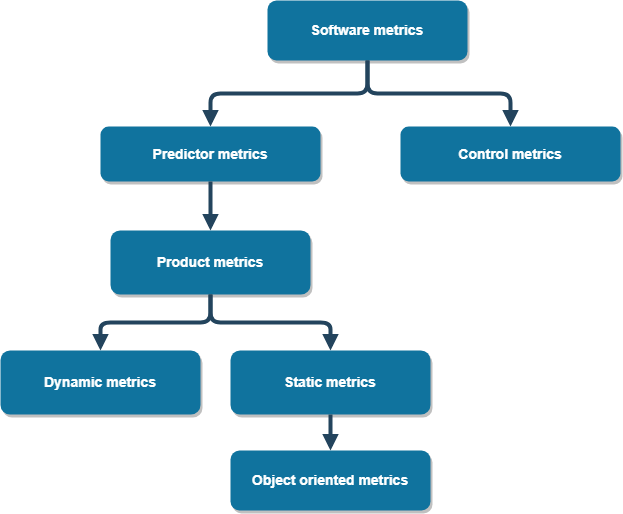
\includegraphics[scale=0.05]{metrictree.png}
\caption{Software metric types}
\label{fig:metrictree}
\end{figure}

\subsection{Product metrics}

Many defined sets of product metrics has been declared in the literature. One defined set is for example Halstead metrics \cite{al2005analysis}. It is also possible to adjust an existing metric for specified software or implement a completely new metric. A product metric can either be dynamic or static \cite{sommerville2011software}. Dynamic metrics are measured when a program is executing and static metrics can be measured for example by reading the source code or documentation of a program. This thesis focuses on static metric analysis. Dynamic metrics such as server uptime are often easy to interpret as 100\% would be the wanted outcome. However, static metrics can often be ambiguous and easily to be misinterpreted. For example SLOC can be 5000 in one product and one million in another. That does not mean that the other is better quality software than the other. This thesis studies static product metrics. Dynamic metrics are also very important for projects, but the company is already using dynamic testing systematically as a tool. Static software analysis has also already been implemented and we focus solely on metrics instead of analyses that for example check common coding practices.

\subsection{Static metrics}

Static metrics can be inspected by comparing the measurement from different files and modules or by plotting metric trend data. Measurements can be ambiguous because the outcome depends from many different factors. For example used programming language is one factor. One interpretation method for static metrics is comparing different results inside the project that is being analyzed. If a part of a software project has anomalous attributes, it should be investigated further. Another method is to define a limit for a good measurement according to literature or just guessing and later adjusting the limit according to own preferences.
When inspecting trend, the magnitude of a static product metric does not matter. Trends of metrics tell if the quality of software is increasing or decreasing to give more profound perceiving of a project.

\subsection{Traditional and object-oriented metrics}

Traditional metrics can be calculated from any kind of software even if the source code is object-oriented. These metrics can be categorized as "non-object-oriented" metrics. Traditional metrics present size of a program and help stake holders to perceive a more accurate picture about what kind of program is being developed. Traditional static metrics are for example SLOC and cyclomatic complexity \cite{fenton1997software}.  

Object-oriented metrics (OOM) are specific for object-oriented programming languages. OOM measurements present structure of a project and tell, for example, if classes are abstract enough for the software to be maintainable. A study has estimated corrective maintenance cost saving to be 42\% when OOM metrics are being used \cite{sarker2005overview}. A good example of OOM metrics are Chidamber and Kemerer Metrics, often referred as CK Metrics \cite{chidamber1994metrics}.

\section{Software quality}
\label{chap:quality}

As bigger and more complex software systems are being developed, the need for quality in these systems has raised. In the 1960s the growth of software projects led to projects lacking maintainability, reusability and reliability \cite{sommerville2011software}. This caused the initiation of different approaches to control software quality in order to make software with less defects and more profit. Defining software quality can be problematic because there exists no one single truth for software quality. Quality has many different attributes such as reliability, security and portability \cite{sommerville2011software}. Every quality attribute can not be taken into account at the same time as improving one attribute of the software can have a decreasing effect on other attribute. Only some of the attributes can be chosen to define if a project has good quality or not. This can lead to conflicts between stakeholders as they can have differentiating points of view and quality attribute preferences about what defines the quality of a software project. Quality management is particularly important for large software systems that takes years to develop. On smaller systems, quality management can be useful but not as mandatory.

\subsection{Software complexity}
\label{chap:complexity}

Structural software complexity measurement is considered as an important factor in software maintainability \cite{banker1989software}. Software has essential complexity that is needed in order to have a functional system and non-essential complexity that is made by accident and can be removed \cite{softcomplex2014}. This means that software must have some level of complexity, but some of the complexity can be removed with refactoring. Unfortunately, complexity is only a number and the amount of non-essential complexity is undefinable. Nevertheless, complexity measurement can hot spot complex parts of a project and indicate, whether complexity is increasing or decreasing. Complex code should be refactored into smaller tasks to make code more understandable and more easily maintainable.  The maintenance of a source code can be two or three times more expensive than the implementation \cite{banker1989software}. Most widely used metric for complexity has been McCabe’s cyclomatic complexity \cite{banker1989software}. Code with high cyclomatic complexity has many independent execute paths and is difficult to understand. 

\begin{figure}[t!]
\centering
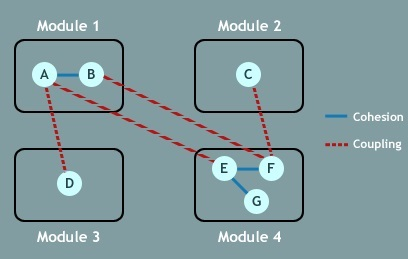
\includegraphics[scale=1]{cohesioncoupling.jpg}
\caption{Cohesion and coupling \protect\cite{cohesion2013poonam}}
\label{fig:cohesioncoupling}
\end{figure}

\subsection{Software modularity}
\label{chap:modularity}

Modularity tells how source code is structured. Modularity is split into relationships between the elements inside a module, cohesion, and relationships between modules, coupling \cite{stevens1999structured}. An example of cohesion and coupling is illustrated in \autoref{fig:cohesioncoupling}. For example module 1 would have one cohesion relationship and three coupling relationships from other modules. Modules can be packages, domains, namespaces or something else, depending which programming language is being used \cite{gupta2009package}.

When structured right, modularity decreases complexity as discussed in \autoref{chap:complexity}. Structured code help developers to change the code later easier as the code is clearly divided in many different modules. Other aspect of modularity is reusability. Modules should be independent as possible to be reusable, meaning that coupling should be as low as possible. If coupling is low, changing an element inside a module means that no other modules must be changed, making the module more independent and reusable. Cohesion inside a module should be high enough to make a module useful. It makes no sense to make many modules that only contains one element because the idea of modularization is to group similar elements together. If modules are independent from other modules, those can be reused in other projects or in other parts of the project while still preserving maintainability. If modules are not independent, changing a piece of a code might change something from other modules and makes refactoring a much more difficult task.

Coupling is divided into two parts: efferent coupling and afferent coupling \cite{gupta2009package}. Efferent coupling means, how many elements from other modules are dependent of the elements inside the module under inspection. Afferent coupling is the opposite, meaning how many elements from inside the inspected module is dependent of outside modules. If module has high efferent and low affarent coupling the module is unstable. High affarent and low efferent coupling means that the module is stable. Instability is not a bad attribute but a module should clearly be either stable or unstable to have a clear meaning \cite{gupta2009package}.


%-Avoiding bugs 
%-complexity = cyclomatic complexity, NPath?
%-reusability (modularity) = affarent, efferent coupling
%-maintainability (readablity) = LOC and what else?





%% CHAPTER 3
\chapter{Determining useful metrics}

Determining the right software metrics is not always a simple task. In this case, the target will be static product metrics. No predefined package of metrics exists that works for every software project. Every project is unique which means that new set of metrics should be selected for each project. However if two projects have a lot in common, the same metrics can be applied. Even after defining metrics, static measurements can be ambiguous due to the fact that the measurement outputs are just numbers. The real correlation of the measurements to the software quality may be easy to misinterpret. The measurement data must be analyzed in order to be able to understand what attributes, if any, it correlates \cite{sommerville2011software}. 

\section{Motivation to implement static analysis}

Quality is an area that ABB want to invest in more and more. Quality product needs, of course, quality software. A certain part of the working effort is allowed to be used for source code refactoring and internal improving. Software metrics analysis will be implemented to help stakeholders to perceive a picture of different quality attributes of the software. The need for software metrics is unclear, but the underlying literature and theory seem to be promising. The idea is to take metrics into use and determine after a short period of usage, if metrics are valuable or not.

%\subsection{Software metrics in agile development process}
%
%The software development team that is the target of this thesis is using an agile software development process. Agile is not a software development process but rather a set of rules that agile %processes try to follow \cite{agilemanifesto}.

\section{Trial and error approach}

As there exists no set of predefined rules that could be used in this context, only logical way is to make a sophisticated guess about what the suitable metrics could be. This can be done iteratively so that chosen metrics are used a defined amount of time and then evaluated again. To do this there must be a way to determine whether the metrics are correlating the wanted attribute or not. One of the goals of this thesis is to implement a first iteration of metrics by choosing metrics according to literature and guessing. The meaning of each chosen metric must be known. If the quality attribute correspondence of a chosen metric is uncertain, it will be impossible to use correctly and will become a number on the board, without meaning.

\subsection{Code smells}

Static software analysis contains possibility to use code smells (see \autoref{chap:sofanatool}). Code smell is a small and fast check for any characteristic that might indicate a software problem \cite{fowlercodesmell}. A smell do not mean that a problem exists but rather that the source code should be reviewed and, if a problem exists, fixed. Code smell usage might be valuable but in a bigger project, so many smells will be present that the few important smells, that are crucial for the project quality, will not be found. Code smells does not add much value when used in daily analysis and should rather be used to check quality on each commit to check smells for the files to be committed \cite{tufano2015and}. This means that code smells are not implemented to the analysis. If needed, a development team should implement a separate code analysis to analyze each commit to the source code. This could be achieved for example with tools like Microsoft Style Cop\footnote{https://github.com/StyleCop/StyleCop}. The goal of this thesis is to implement a static software analysis which is run daily and not on each commit. Code smells will not be implemented to the analysis. 

\subsection{Complexity metrics}

Three complexity metrics will be selected to analyze maintainability (see: \autoref{chap:complexity}) from different points of view. Cyclomatic complexity is a widely used metric that tells number of ways that a program can be executed. It is a good way to see, for example, if a part of a program  has a complex switch sentence or something similar, that is difficult to read.
Maintainability index is a number that is a combination of different metrics that has been stated to correlate maintainability well. This metric is the most unambiguous metric that is being selected because a higher number means better maintainability. Maintainability index helps less experienced programmers to understand, whether complexity is increasing or decreasing. Third is duplicate code which tells percentage of code duplications in the code base. If, for example, a method is found in two different places, changing of that method means that the change must be implemented twice.

\begin{table}[t!]
\centering
\caption{The chosen metrics}
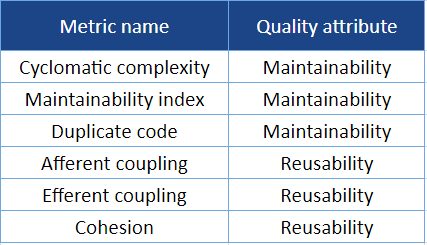
\includegraphics[scale=1]{metrics.png}
\label{fig:metrics}
\end{table}

\subsection{Modularity metrics}

Also three metrics that tend to correlate modularity, are being selected. Afferent and efferent coupling (see \autoref{chap:modularity}) will tell how mixed the modules are. Modules should have low coupling and they should be either stable or instable as possible. Coupling will be inspected in module level but could also be analyzed for class level to see how stable or instable individual classes are. Class level coupling however, is not selected as core metrics in this case. Cohesion means total coupling between classes inside each module. If cohesion is low, the inspected module might be useless meaning that either more elements must be added or the few elements that the module has, must be moved elsewhere. These three metrics can be very ambiguous if not understood correctly. Modular refactoring can be very laborious and might be almost impossible or too much of a time waste, if the project is big and heavily coupled. However it might offer a big improvement concerning reusability and maintainability. The chosen metrics and their main corresponding attributes are listed in \autoref{fig:metrics}. The metrics may correspond to other quality attributes aswell. 

\section{Source code examples}
To really test if the metrics are correlating the wanted software quality attributes, low and high quality source code examples are needed to be determined \cite{coleman1994using}. These examples should be good or bad quality code according to the whole development teams opinion. After good and bad quality has been concretely defined, figuring out which metrics correlate to the quality can be initiated. 




%% CHAPTER 4
\chapter{Implementing analysis for a development team}

After making sure that the software metrics really are useful and capable of indicating software quality it is time to make use of the metrics. In this chapter a proof of concept will be implemented and possibly introduced for the use of a software development team.

\section{Essential tools for implementation}

For a concrete implementation, some software tools are needed. The preference is that metrics are easily visible and understandable for each developer. Metrics are not meant to be a stressing factor which might happen if the metrics are forced to be seen on a day-to-day basis. Metrics should rather be an auxiliary tool to help developers perceive a bigger picture regarding source code. No comparison was done while choosing the tools and the main idea is to use tools that are easily available or already in use by the company.

\subsection{Software analysis tool}
\label{chap:sofanatool}

CppDepend\footnote{https://www.cppdepend.com/} is a commercial tool specifically made to analyze C/C++ code. It provides many of the common software metrics and has a good-looking user interface. There are many other promising tools but investigating available options is out of scope on this thesis. Using this tool gives a good indication if software metrics are useful for the software development team or not. If the tool later turns out to be exchangeable with a more usable one, it can easily be replaced.

\subsection{Analysis automation tool}

Jenkins\footnote{https://jenkins.io/} is an open-source continuous integration tool. Jenkins is a server that can easily be set to trigger for example CppDepend to analyze source code daily. It can also be set to store artifacts which in this case would be the analysis outcome in Hypertext Markup Language (HTML) format.  The strength of Jenkins is that anyone in the research and development department who has access to the internet can observe the outcome of the analysis. Source code is updated to the latest version with the help of Git\footnote{https://git-scm.com/}. Git is a distributed version control system that is widely used all over the world \cite{gitsurvey}.

\subsection{Build server}

Analysis can not be done on any computer. It must be a computer that is constantly powered on and online. This way the analysis will be run constantly and enables continuous data for different graphs. For this purpose a build server will be set up. Jenkins will be connected to this computer and will tell the server to do the required commands. A local copy of the source code is stored in the server and it will always have the latest version of the software available by using Git before any analysis.

\begin{figure}[t!]
\centering
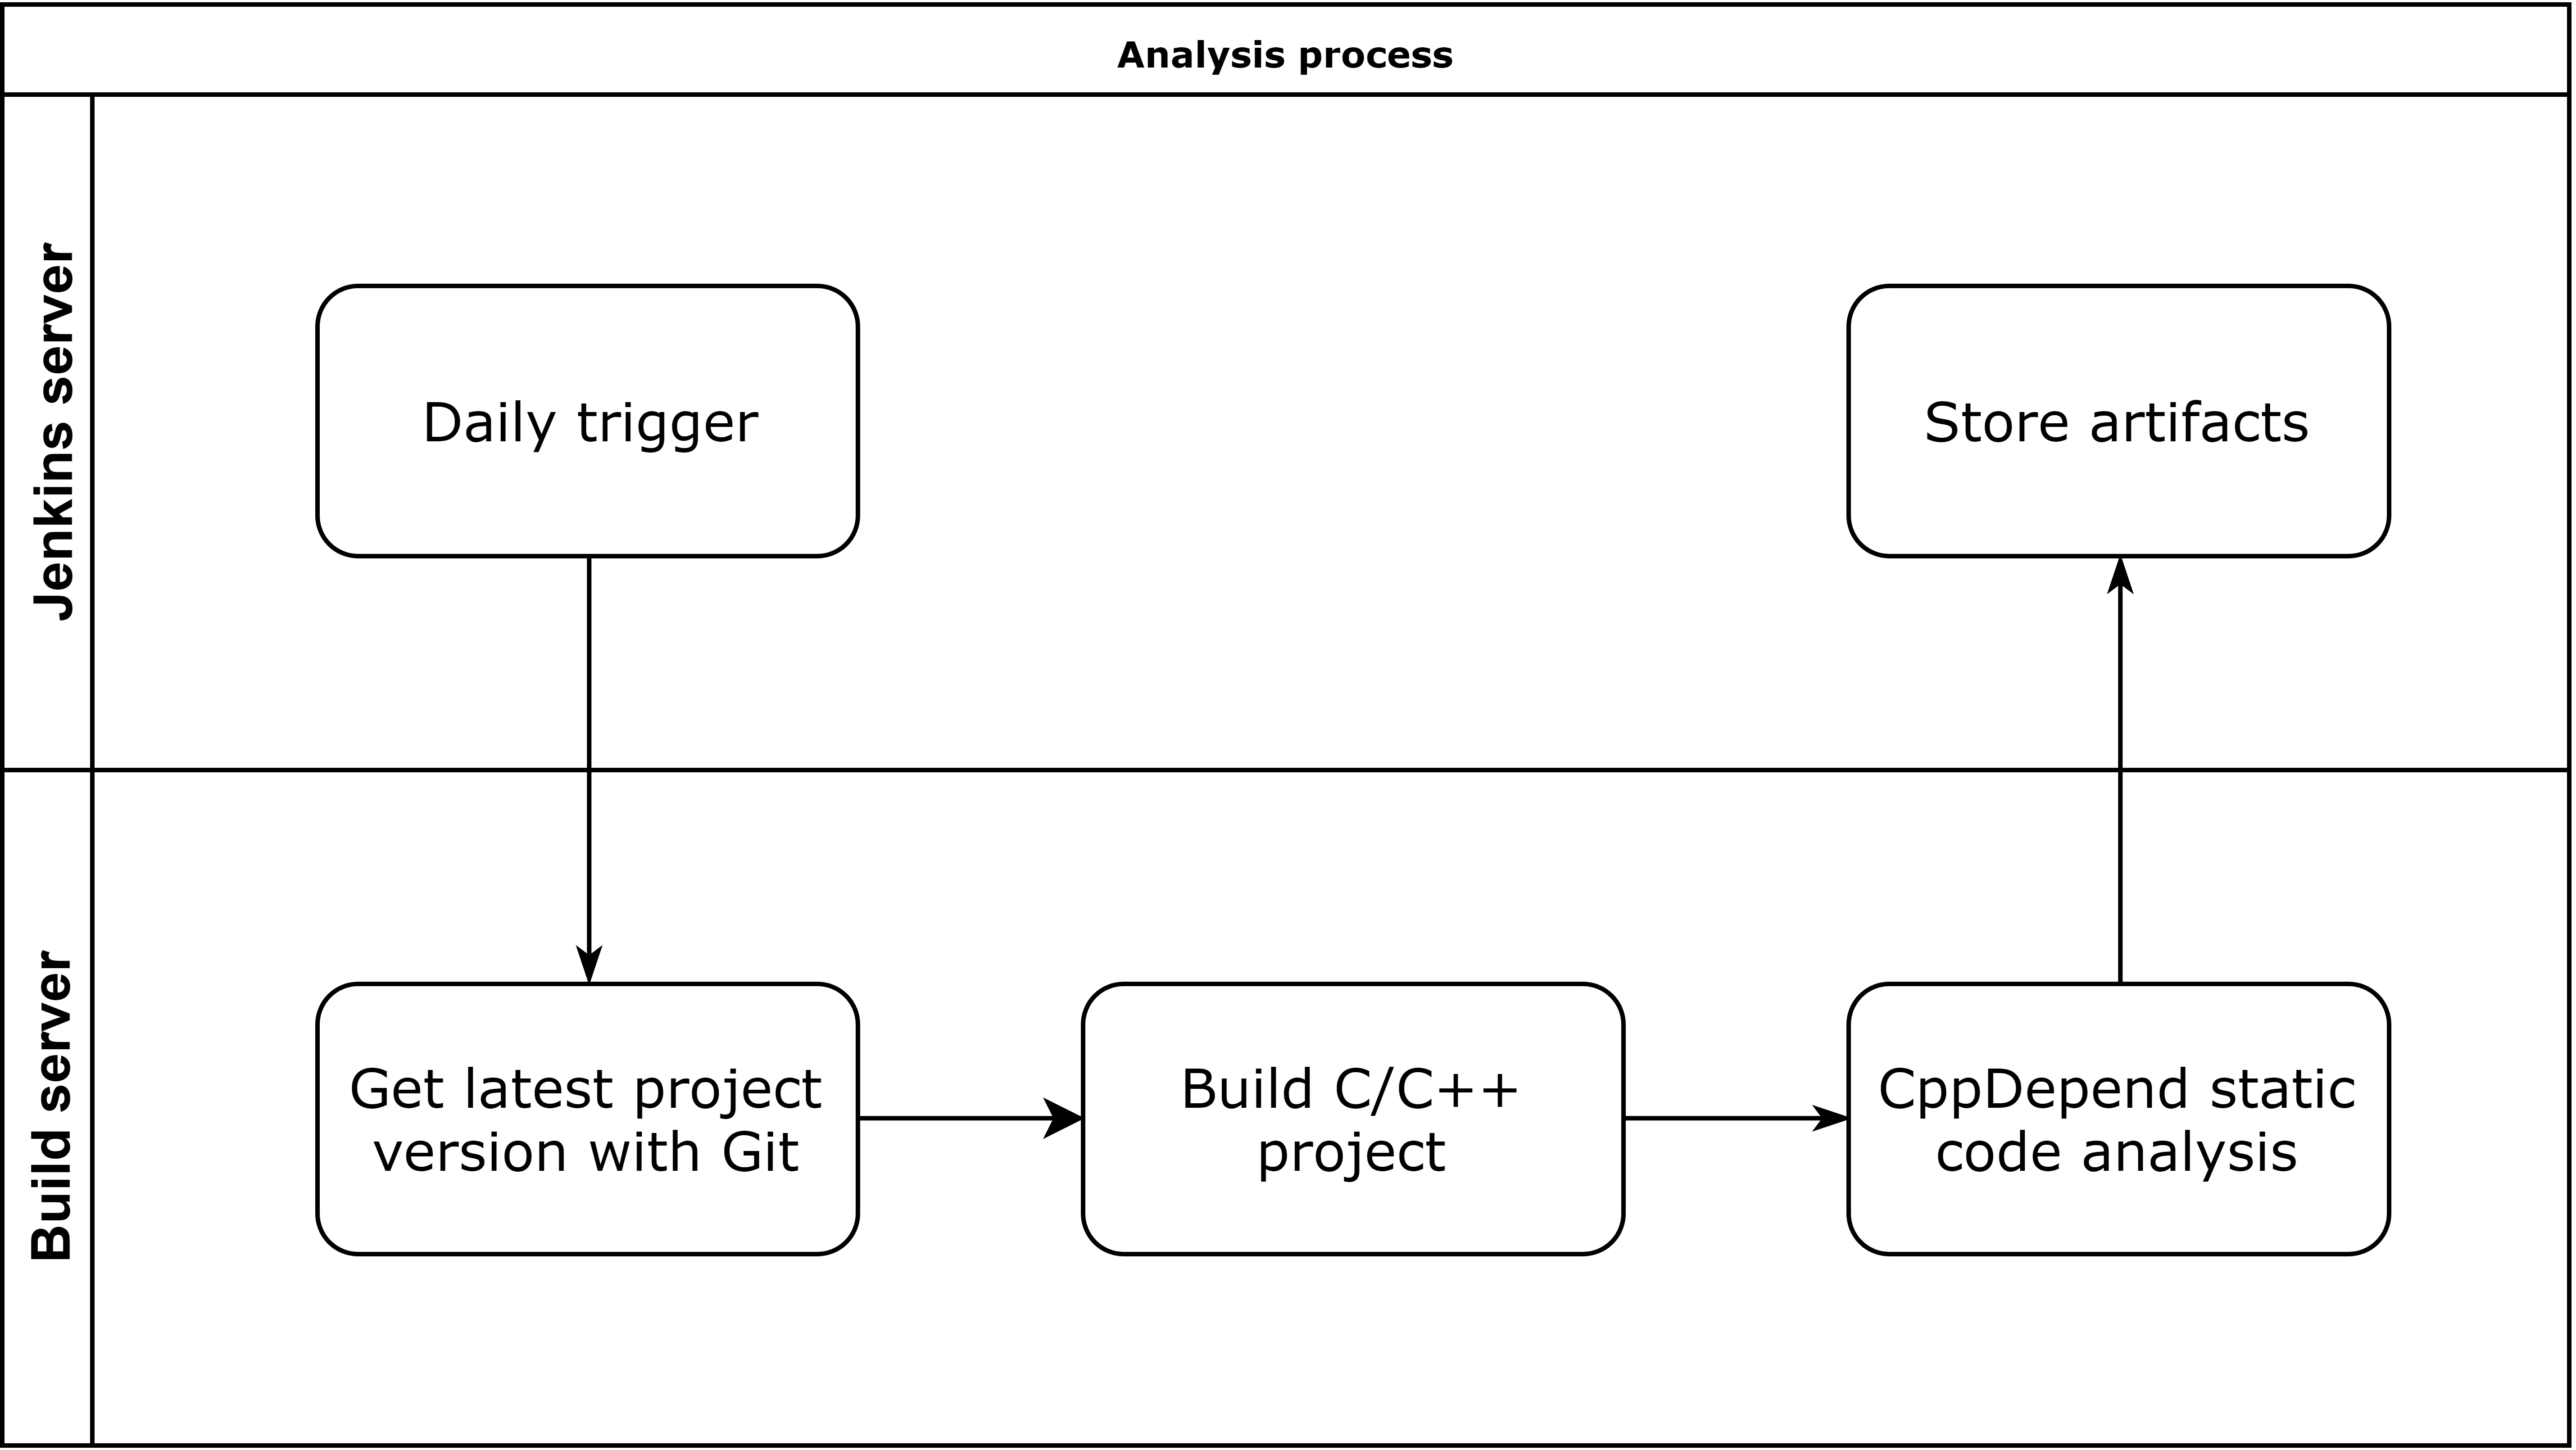
\includegraphics[scale=0.06]{systemdesc.png}
\caption{System funcionality}
\label{fig:systemdesc}
\end{figure}

\section{System description}

The selected tools will form a system that will create desired analysis daily to the Jenkins server where it can be inspected by everyone. The system functionality is illustrated in figure~\ref{fig:systemdesc}. Jenkins can be set to periodically call a sequence of commands. In this case, the period will be one day. The source code will be upgraded to its latest version with version control system, Git. After the source code is upgraded, it will be compiled and analyzed by the CppDepend tools. CppDepend will return analysis artifacts as a HTML file to the Jenkins server, which will be stored and viewable in the Jenkins user interface.
This way the process will be transparent and available to the whole software development team.

The whole process takes only about ten minutes to run and is not a strenuous task for the build server. The analysis tool does an incremental analysis, which means that if some part of the source code is not changed, it will be copied from the last report and not analyzed again.





%% CHAPTER 5
\chapter{Conclusions}

Quality is a big concern in large software projects that take long time to develop.
It has become clear that software metrics are an important factor in the modern software development business. Software metrics are not very widely studied and the needed metrics differ on each project and company. 

\section{What is needed}

The software development department is concerned with the overall quality of software projects. It takes time to understand poorly written and structured code. Refactoring can help to make the code base more understandable and maintainable and to ensure that complexity does not get out of control. This is a huge concern, as the software that is being developed is supposed to be supported many years, or even decades, to come. Static software analysis is one way to help developers and management to perceive a better and more clear picture of the code base. This possibly help to highlight the most poorly structured code that potentially does the most harm when maintainability is concerned.

\section{What is done}

Six core software metrics that could be useful for analysis have been chosen to help analyze complexity and modularity of code base. The metrics are ambiguous in a way that the pure measurement numbers alone do not tell anything. Who ever is reading the analysis, needs a more profound understanding of the collected software metrics in order to not to make false conclusions. Moreover, the analysis has been implemented to the common infrastructure of the software teams to make the analysis easily accessible. The analysis is scheduled to run daily to make the analysis always have the latest data and to be able to plot metric trends. Other software metrics and trend data is being analyzed as well but the usefulness of those metrics and especially the code smells is not certain and might just confuse developers. This thesis was written in three months, which is a small time for a big company. The usefulness of the chosen metrics and tools could not be tested in such a short period of time. This thesis has however started the usage of clearly structured static product metrics.

\section{Actions in the future}


In the future, the company can analyze output data of the made static software analysis and possibly decide common quality standards for software development. Many projects inside the software development department have similar structures and quality attribute preferences which helps the project teams to compare some of the metrics and, perhaps, imitate processes that are born with the static analysis. The next step could be to implement the static analysis for other development teams as well. This is made easier by making the scripts and Jenkins configurations easy to modify and to implement on different projects.


%%  LIITTEET  ------------------------------------------

\bibliographystyle{apacite}
\bibliography{references}

\end{document}
